\documentclass[]{article}

\usepackage[english]{babel}
\usepackage{graphicx}
\usepackage{booktabs}
\usepackage{float}
\usepackage{hyperref}

\title{A Bidirectional LSTM Model for Recalling Jokes Using Word Embeddings}
\author{Juan Lao Tebar}

\begin{document}
	\maketitle
	
	\section{Introduction}
	
	Humour is the disposition of certain cognitive experiences to cause laughter and produce enjoyment, a complex process difficult to analyze from a scientific point of view. Many hypothesis try to explain what humour is, how it works, or what social function it serves. For example, Peter McGraw, 2012 states that ``humour only occurs when something seems wrong, unsettling, or threatening, but simultaneously seems okay, acceptable or safe’’.
	
	Humour can be verbal, visual or physical, but no matter the form there is a complex underlying relation between the elements that basically manifest a reflexion, an imitation, a surprise, a paradox, an ambiguity or an exaggeration. These concepts are presented with particular methods of different degrees of complexity, such as metaphors or hyperboles.
	
	In particular, jokes are verbal representations of humour that, in the linguistic plane, consist of complex constructions that play not only with the objective meaning of the terms but also with the subjective interpretation and culture of the interlocutors.
	
	Word embeddings are good representations of the semantic meaning of linguistic terms, associating words with descriptive numerical vectors. By defining a distance function between those vectors, we can find solid logical relations between them.
	
	In this practice we analyze the behavior of a model that uses word embeddings for generating jokes.
	
	Our model is a sequence-to-sequence bidirectional LSTM neural network trained with a Question-Answers Jokes dataset\footnote{\url{https://www.kaggle.com/jiriroz/qa-jokes}} consisting of 38,269 jokes from Reddit. The input of the model is a question and the output is a---relatively---funny answer. The main objective of our work is to play with different configurations of embedding sources and sizes in order to extract some conclusions about them, thus we do not to focus on the details and fine-tuning of the network.
	
	It is very difficult to generate new jokes, even as a human. Before starting working on this practice we attempted to train the model with common cross-validation, but we found that it was not possible to decrease the validation loss at all, even applying regularization methods. Our model can learn a lot of jokes from a particular training set, but it cannot generalize the \emph{humour sense} to create new jokes. For this reason we decided to focus this practice on teaching the model some jokes and playing later with the meaning and sense of the questions and answers, checking what happens when we change the original words by similar alternatives, or what happens when we replace some words following a semantic regularity (e.g., changing the gender of the subject).
	
	The word embeddings we use come from different sources: GloVe\footnote{\url{https://nlp.stanford.edu/projects/glove/}}, word2vec\footnote{\url{https://code.google.com/archive/p/word2vec/}} and LexVec\footnote{\url{https://github.com/alexandres/lexvec}}. Each provider offers different pre-trained versions, trained with different corpus, with different vector dimensions.
	
	This dataset contains jokes that can be considered inappropriate, irrespectful or offensive for certain collectives. We do not share the point of view of the people who created these jokes.
	
	The code related to this work is public and available at github\footnote{\url{https://github.com/juanlao7/reddit_qajokes-BLSTM}}.
	
	\section{Report}
	
	\subsection{Description of the Model}
	
	From the original dataset we use only jokes with a maximum question size of 19 words and a maximum answer size of 17 words.
	
	Our model takes as an input a sequence of 19 embedded words and gives as output a sequence of 17 embedded words. Inputs and outputs with a lesser length are padded with a \emph{padding token} vector until they have size 17. If a joke of the dataset contains a word that cannot be found in the embedding dictionary, then the joke is discarded.
	
	The neural network has a bidirectional LSTM layer of 128 units with an hyperbolic tangent activation for encoding the input, and another bidirectional LSTM of 128 units with also hyperbolic tangent activation for decoding the output. Finally, these hidden units are connected to a dense linear output layer.
	
	We train the model with RMSprop, with a learning rate of 0.001, $ \rho = 0.9 $, $ \varepsilon = 1 \cdot 10^{-8} $ and no learning rate decay.
	
	As previously said, in this practice we do not validate or test our model. We just train it for 200 epochs and then we analyze the result. The loss is calculated with the Mean Square Error (MSE), since we want to reduce the distance between our output and the target embedding vectors.
	
	When the model gives an output in the form of a sequence of word embeddings, we can obtain a textual representation of the answer by finding the nearest neighbor of each vector. For this purpose we use an implementation of a K-D tree, where the cost of finding the nearest neighbors of a term is logarithmic.
	
	\subsection{Word Pre-processing}
	
	In order to train the model, we must first convert all the original jokes into sequences of embedded words, using the embedding dictionaries provided by each source of embedding vectors.
	
	Unfortunately, the jokes from the dataset contain contractions (``what’s’’, ``father’s’’, ``you’re’’), words written in different cases (``What’’, ``what’’, ``WHAT’’) or symbols (``?’’, ``!’’, ``.’’, ``,’’). In order to represent as many words as possible, we perform a pre-processing over each joke, that consists in the following:
	
	We convert the original text into lowercase.
	We remove all the characters that are not numbers, letters or spaces.
	All the words in the joke---question and answer---must consist only of letters, numbers or start with a number and then follow with only letters (e.g., ``18cm’’). In other case, we discard the joke.
	
	We apply the same process to the embedding dictionary, removing contractions and non-alphanumeric symbols from the keys and discarding those that do not meet the condition described in step 3.
	
	With this process we aim to increase the size of the intersection between the vocabulary of the dataset and the chosen embedding set.
	
	\subsection{Padding Tokens}
	
	As previously said, there are different ways of representing the \emph{padding token}, and it directly affects the performance of the model:
	
	\begin{enumerate}
		\item A vector where all components are zero.
		\item A vector where each component $ i $ is equal to $ m_i + 2 \cdot s_i $, where $ m_i $ is the mean value that component $ i $ takes among all the words of the embedding space and $ s_i $ is the standard deviation.
		\item Same as the previous approach, but each component $ i $ is equal to $ m_i + 3 \cdot s_i $.
		\item We add a new extra component to all the embedding vectors. For the embedded words its value is zero, but for the padding token is 1 and the rest of the components are zero. In this case, when we need to obtain the textual representation of the output of our network, we define a threshold on the extra dimension to determine if an output is a padding token. If this threshold is not reached, then we obtain the nearest neighbor in the embedding space based on the original vector dimensions. In our experiments we found that the optimal threshold that minimizes false positives and false negatives is 0.2.
	\end{enumerate}
	
	In this experiment we test all the different ways of defining the padding token vector on GloVe---trained with 6 billion tokens, 300 dimensions---, and we compute the error of the models when determining if an embedded word is a padding token or not---number of false positives and false negatives.
	
	Table \ref{t:tokens} shows the average error when predicting the padding token on the first 50 answers of the dataset.
	
	\begin{table}[H]
		\centering
		\begin{tabular}{@{}cc@{}}
			\toprule
			Encoding method		  & Error \\ \midrule
			0s                    & $0.66 \pm 1.51$              \\
			Extra dimension       & $0.64 \pm 1.49$              \\
			2 standard deviations & $0.76 \pm 1.90$              \\
			3 standard deviations & $0.92 \pm 2.39$              \\ \bottomrule
		\end{tabular}
		\caption{Average error when predicting the padding token on the first 50 answers of the dataset.}
		\label{t:tokens}
	\end{table}
	
	As we can see, the extra dimension method has the lowest error. In the following experiments we use this method for encoding the padding tokens.
	
	\subsection{Differences Between Embedding Sizes}
	
	When the training process in certain models takes too much memory or too much time to converge, using less dimensions to represent the embedded words may be a good option to consider in exchange of losing representational power.
	
	Our model does not suffer from any of these problems, but it is interesting to observe how the embedding size affects the results. In this experiment we test GloVe trained with 6 billion tokens with 50, 100, 200 and 300 dimensions.
	
	As we can see in figure \ref{f:sizes}, more dimensions lead to a lower MSE. However, it is difficult to extract a conclusion from this fact, since the output of our network is an embedded word and comparing the MSE between models makes no sense. The embeddings have been trained using different neural networks, thus we can not guarantee that the embedding spaces they approximated have anything in common.
	
	\begin{figure}[H]
		\centering
		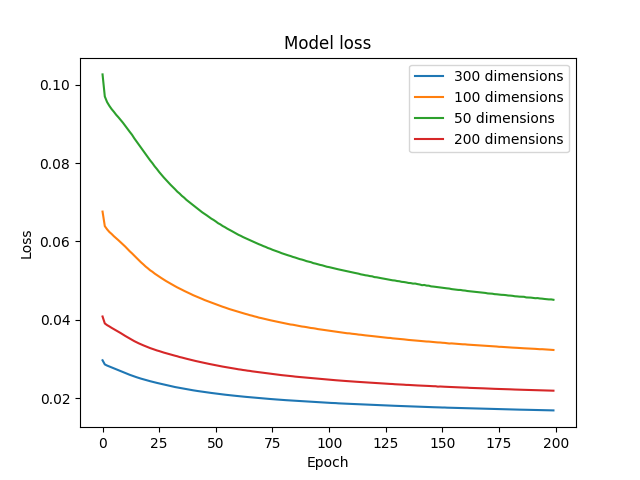
\includegraphics[width=0.5\textwidth]{sizes}
		\caption{Training loss with each embedding size.}
		\label{f:sizes}
	\end{figure}
	
	To be able to analyze the results, we need to compare the textual representations of their output---number of correctly predicted tokens divided by 17, the answer length---. Table \ref{t:sizes} shows the global accuracy of each approach on predicting the correct word.
	
	\begin{table}[H]
		\centering
		\begin{tabular}{@{}cc@{}}
			\toprule
			Dimensions & Accuracy            \\ \midrule
			50         & $0.7694 \pm 0.1758$ \\
			100        & $0.7688 \pm 0.1734$ \\
			200        & $0.7771 \pm 0.1673$ \\
			300        & $0.7829 \pm 0.1690$ \\ \bottomrule
		\end{tabular}
		\caption{Textual representation accuracy for each embedding size.}
		\label{t:sizes}
	\end{table}
	
	\subsection{Differences Between Corpus}
	
	GloVe word embeddings have been obtained from different corpus, resulting in a different number of words in each case. In particular, there is a package trained with 6 billion tokens extracted from Wikipedia 2014 + Gigaword 5 resulting in 400,000 words, and another trained with 42 billion tokens from Common Crawl resulting in 1.9 million words.
	
	Increasing the number of words in the embedding space should not affect the loss of the model, but probably will decrease the accuracy of the textual representation, due to recalling very close wrong neighbors. In this experiment we train and compare the results of two models, one trained with the 400,000 word set and other with the 1.9 million.
	
	Figure \ref{f:corpus} shows the MSE evolution through the training, while table \ref{t:corpus} shows the textual representation accuracy of each.
	
	\begin{figure}[H]
		\centering
		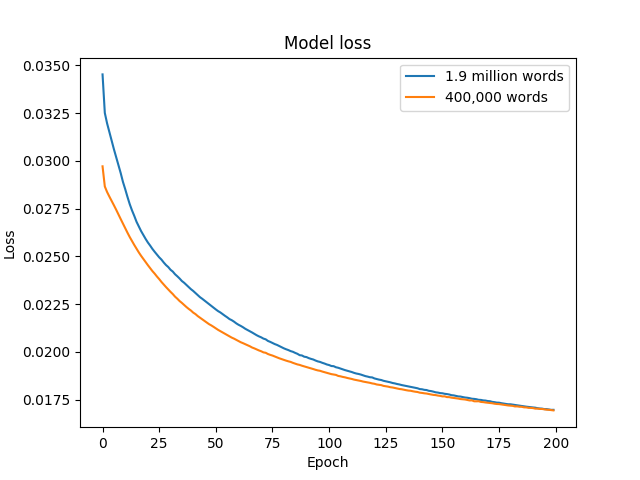
\includegraphics[width=0.5\textwidth]{corpus}
		\caption{Training loss with each corpus.}
		\label{f:corpus}
	\end{figure}
	
	\begin{table}[H]
		\centering
		\begin{tabular}{@{}cc@{}}
			\toprule
			Words       & Accuracy            \\ \midrule
			400,000     & $0.7829 \pm 0.1690$ \\
			1.9 million & $0.7700 \pm 0.1557$ \\ \bottomrule
		\end{tabular}
		\caption{Textual representation accuracy for each corpus.}
		\label{t:corpus}
	\end{table}
	
	Table \ref{t:corpus2} shows some examples where the model trained with the small set got better results than the bigger.
	
	\begin{table}[H]
		\centering
		\begin{tabular}{@{}cccc@{}}
			\toprule
			Question                                                                                                     & Answer                                                                        & 400,000 words                                                                       & 1.9 million words                                                                                                                \\ \midrule
			\begin{tabular}[c]{@{}c@{}}why was the\\ router released\\ early from prison?\end{tabular}                   & it had connections                                                            & it \textbf{had} srivalo                                                                      & it \textbf{was} assmtsale                                                                                                                 \\ \midrule
			\begin{tabular}[c]{@{}c@{}}why do black\\ people like\\ korean food?\end{tabular}                            & \begin{tabular}[c]{@{}c@{}}because it has\\ a little seoul in it\end{tabular} & \begin{tabular}[c]{@{}c@{}}because it have\\ a but bulletinyyy\\ \textbf{in} it\end{tabular} & \begin{tabular}[c]{@{}c@{}}because it was\\ a though\\ nowupload \textbf{both} it\end{tabular}                                            \\ \midrule
			\begin{tabular}[c]{@{}c@{}}what did the\\ atheist fisherman\\ say when asked\\ about his catch?\end{tabular} & there is no cod                                                               & \textbf{there is} but                                                                        & \begin{tabular}[c]{@{}c@{}}\textbf{because it} even\\ bmxznot\end{tabular}                                                                \\ \bottomrule
		\end{tabular}
		\caption{Outputs of the model trained with each corpus.}
		\label{t:corpus2}
	\end{table}
	
	\subsection{Differences Between Embedding Algorithms}
	
	While GloVe creates its embeddings by aggregating global word-word co-occurrence statistics from a corpus, other algorithms such as word2vec implement continuous bag-of-words and skip-gram architectures for computing vector representations of words, and others like LexVec use low-rank, weighted factorization of the Positive Point-wise Mutual Information matrix via stochastic gradient descent.
	
	In this experiment we train our model with the following embeddings:
	
	\begin{description}
		\item[GloVe:] Corpus from Common Crawl, 42 billion tokens, 1.9 million words, 300 dimensions.
		\item[word2vec:] Corpus from Google News, 100 billion tokens, 3 million words, 300 dimensions.
		\item[LexVec:] Corpus from Common Crawl, 58 billion tokens, 2 million words, 300 dimensions.
	\end{description}
	
	Figure \ref{f:sources} shows the MSE evolution through the training, while table \ref{t:sources} shows the textual representation accuracy of each.
	
	\begin{figure}[H]
		\centering
		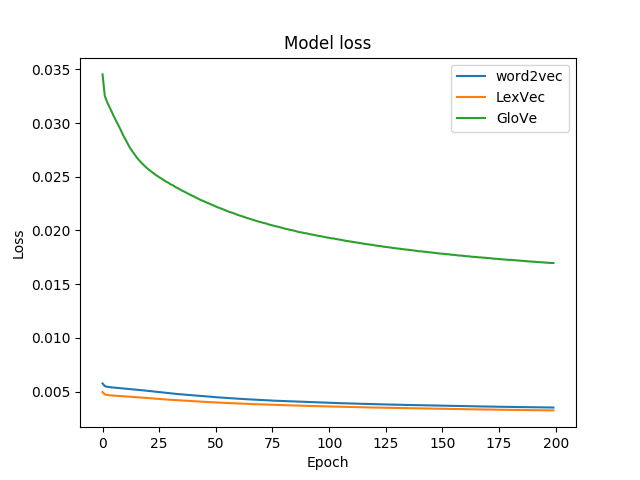
\includegraphics[width=0.5\textwidth]{sources}
		\caption{Training loss with each embedding embedding algorithm.}
		\label{f:sources}
	\end{figure}
	
	\begin{table}[H]
		\centering
		\begin{tabular}{@{}cc@{}}
			\toprule
			Algorithm & Accuracy            \\ \midrule
			GloVe     & $0.7700 \pm 0.1557$ \\
			word2vec  & $0.7424 \pm 0.1672$ \\
			LexVec    & $0.7482 \pm 0.1596$ \\ \bottomrule
		\end{tabular}
		\caption{Textual representation accuracy for each embedding algorithm.}
		\label{t:sources}
	\end{table}
	
	As we can see, GloVe offers the best textual accuracy in our case.
	
	\subsection{Results}
	
	At this point we regret to say that our best model---trained with GloVe 6B 300---offers very poor results. Table \ref{t:examples} shows a variety of answers given by the network.
	
	\begin{table}[H]
		\centering
		\begin{tabular}{@{}ccc@{}}
			\toprule
			Question                                                                                        & Actual answer                                                                              & Model prediction                                                                                                                \\ \midrule
			\begin{tabular}[c]{@{}c@{}}why are frogs\\ so happy?\end{tabular}                               & \begin{tabular}[c]{@{}c@{}}they eat whatever\\ bugs them\end{tabular}                      & \begin{tabular}[c]{@{}c@{}}they they anyway\\ httpwwwmediabynumberscom\\ even\end{tabular}                                      \\ \midrule
			\begin{tabular}[c]{@{}c@{}}why did the\\ hipster burn\\ his tongue?\end{tabular}                & \begin{tabular}[c]{@{}c@{}}because he drank\\ his coffee before\\ it was cool\end{tabular} & \begin{tabular}[c]{@{}c@{}}because he ate\\ he instance before\\ it was cool\end{tabular}                                       \\ \midrule
			\begin{tabular}[c]{@{}c@{}}whats brown\\ and sticky?\end{tabular}                               & a stick                                                                                    & a stick                                                                                                                         \\ \midrule
			\begin{tabular}[c]{@{}c@{}}why did mozart\\ kill his chickens?\end{tabular}                     & \begin{tabular}[c]{@{}c@{}}they were yelling\\ bach bach bach bach\end{tabular}            & \begin{tabular}[c]{@{}c@{}}they were piyanart\\ bulletinyyy bulletinyyy\end{tabular}                                            \\ \midrule
			\begin{tabular}[c]{@{}c@{}}which came first\\ the chicken or\\ the egg?\end{tabular}            & the rooster                                                                                & the the bulletinyyy                                                                                                             \\ \midrule
			\begin{tabular}[c]{@{}c@{}}who put semen\\ in the basement?\end{tabular}                        & \begin{tabular}[c]{@{}c@{}}i dont know\\ thats just the\\ way its spelled\end{tabular}     & \begin{tabular}[c]{@{}c@{}}i dont know\\ oooooooooooooooooo--\\ ooooooooooooooooooooo\\ so indeed but\\ but bulletinyyy\end{tabular} \\ \midrule
			\begin{tabular}[c]{@{}c@{}}what do you\\ do when your\\ wife starts smoking?\end{tabular}       & \begin{tabular}[c]{@{}c@{}}slow down\\ and apply lube\end{tabular}                         & \begin{tabular}[c]{@{}c@{}}coming put and\\ instance\\ oooooooooooooooooo--\\ ooooooooooooooooooooo\end{tabular}                     \\ \midrule
			\begin{tabular}[c]{@{}c@{}}what is statistically\\ three times worse\\ than a war?\end{tabular} & three wars                                                                                 & three piyanart                                                                                                                  \\ \midrule
			\begin{tabular}[c]{@{}c@{}}why dont drug\\ addicts hang out\\ at the beach?\end{tabular}        & \begin{tabular}[c]{@{}c@{}}they dont like\\ getting sand in\\ their crack\end{tabular}     & \begin{tabular}[c]{@{}c@{}}they dont so\\ so bulletinyyy in\\ their bulletinyyy\end{tabular}                                    \\ \midrule
			\begin{tabular}[c]{@{}c@{}}how does a\\ jew make his\\ coffee?\end{tabular}                     & hebrews it                                                                                 & hebrews it                                                                                                                      \\ \bottomrule
		\end{tabular}
		\caption{Some model outputs.}
		\label{t:examples}
	\end{table}
	
	As we can see, in some cases the model recalls the full answer to the question, but in the majority of them it does not give even a syntactically correct output. Some words are incorrectly recalled with a high frequency (e.g. ``bulletinyyy’’, ``ooooooooooooooooooooooooooooooooooooooo’’), probably because they are very close to the padding token.
	
	One interesting thing we can observe is that the model usually outputs the right number of words, even if they are wrong. Looks like the network easily learns and focus on the number of padding tokens it must output at the end of the sentences.
	
	\subsection{Playing with Semantic Regularities}
	
	Our model \emph{memorizes} the answers to the questions, but what happens if we replace a word in the question with a regularity? Does the model output an answer that also uses the regularity?
	
	In GloVe---trained with 6 billion tokens, 300 dimensions---we can find several regularities, as shown in tables \ref{t:reg1}, \ref{t:reg2} and \ref{t:reg3}.
	
	\begin{table}[H]
		\centering
		\resizebox{\textwidth}{!}{%
		\begin{tabular}{@{}ccc@{}}
			\toprule
			hitler $-$ germany + italy & hitler $-$ germany + russia & hitler $-$ germany + cuba \\ \midrule
			mussolini                & stalin                    & cuba                    \\
			hitler                   & hitler                    & fidel                   \\
			italy                    & russia                    & castro                  \\
			adolf                    & kremlin                   & cuban                   \\
			fascist                  & putin                     & havana                  \\ \bottomrule
		\end{tabular}%
		}
		\caption{A regularity between dictators and the countries under their power.}
		\label{t:reg1}
	\end{table}
	
	\begin{table}[H]
		\centering
		\resizebox{\textwidth}{!}{%
		\begin{tabular}{@{}ccc@{}}
			\toprule
			merkel $-$ germany + spain & merkel $-$ germany + italy & merkel $-$ germany + france \\ \midrule
			aznar                    & berlusconi               & sarkozy                   \\
			zapatero                 & prodi                    & chirac                    \\
			sarkozy                  & merkel                   & merkel                    \\
			merkel                   & sarkozy                  & fillon                    \\
			spain                    & italy                    & france                    \\ \bottomrule
		\end{tabular}%
		}
		\caption{A regularity between presidents and the countries they preside.}
		\label{t:reg2}
	\end{table}
	
	\begin{table}[H]
		\centering
		\begin{tabular}{@{}ccc@{}}
			\toprule
			dad $-$ man + woman & uncle $-$ man + woman & grandfather $-$ man + woman \\ \midrule
			mom             & aunt              & grandmother             \\
			dad             & niece             & grandfather             \\
			mother          & uncle             & granddaughter           \\
			grandmother     & grandmother       & mother                  \\
			widowed         & mother            & niece                   \\ \bottomrule
		\end{tabular}
		\caption{A regularity between family relationship and gender.}
		\label{t:reg3}
	\end{table}
	
	We tried to find jokes where we can apply those regularities, but in the majority of cases the model is unable to learn the answer, making impossible to apply them, as shown in table \ref{t:reg4}. In the case of the presidency regularity we could not find any joke in the dataset that involves merkel \& germany, aznar \& spain, berlusconi \& italy or sarkozy \& france.
	
	\begin{table}[H]
		\centering
		\begin{tabular}{@{}ccc@{}}
			\toprule
			Question                                                                                        & Actual answer                                                                              & Model prediction                                                                                               
			\\ \midrule
			\begin{tabular}[c]{@{}c@{}}how did hitler\\ originally get\\ into power?\end{tabular}                         & \begin{tabular}[c]{@{}c@{}}lets make\\ germany great\\ again\end{tabular}                                                         & piyanart it but but                                                                                                                                                                                             \\ \midrule
			\begin{tabular}[c]{@{}c@{}}why did russia\\ lose the race?\end{tabular}                                       & \begin{tabular}[c]{@{}c@{}}because it was\\ stalin edit sorry\\ communist jokes arent\\ funny unless every\\ gets them\end{tabular} & \begin{tabular}[c]{@{}c@{}}because he was\\ bulletinyyy\\ oooooooooooooooooo--\\ ooooooooooooooooooooo\\ bulletinyyy indeed\\ bulletinyyy\\ httpwwwmediabynumberscom\\ indeed actually even piyanart so\end{tabular} \\ \midrule
			\begin{tabular}[c]{@{}c@{}}why did russia\\ sign the\\ nonaggression\\ pact with nazi\\ germany?\end{tabular} & \begin{tabular}[c]{@{}c@{}}they were stalin\\ for time\end{tabular}                                                               & \begin{tabular}[c]{@{}c@{}}they were\\ bulletinyyy\\ same but\end{tabular}                                                                                                                                      \\ \midrule
			\begin{tabular}[c]{@{}c@{}}why are cars\\ in russia so slow?\end{tabular}                                     & \begin{tabular}[c]{@{}c@{}}because they are\\ always stalin\end{tabular}                                                          & \begin{tabular}[c]{@{}c@{}}because they are\\ so\end{tabular}                                                                                                                                                   \\ \midrule
			\begin{tabular}[c]{@{}c@{}}why didnt anyone\\ drive stick in\\ soviet russia?\end{tabular}                    & \begin{tabular}[c]{@{}c@{}}they were afraid\\ of stalin\end{tabular}                                                              & \begin{tabular}[c]{@{}c@{}}they were indeed\\ of\end{tabular}                                                                                                                                                   \\ \bottomrule
		\end{tabular}
		\caption{All the jokes that contain hitler \& germany, mussolini \& italy, stalin \& russia or castro \& cuba. The model is unable to recall the important words.}
		\label{t:reg4}
	\end{table}
	
	Table \ref{t:reg5} shows some cases where the model gives an answer where the regularity is applicable. This happens only on the gender and family relationship regularity.
	
	Table \ref{t:reg6} shows the results after replacing the question applying the regularity.
	
	\begin{table}[H]
		\centering
		\begin{tabular}{@{}ccc@{}}
			\toprule
			Question                                                                                                      & Actual answer                                                                                  & Model prediction                                                                                                                  \\ \midrule
			\begin{tabular}[c]{@{}c@{}}whats the difference\\ between me and\\ your mom?\end{tabular}                     & \begin{tabular}[c]{@{}c@{}}your mom hasnt\\ had sex with\\ your mom\end{tabular}               & \begin{tabular}[c]{@{}c@{}}your mom\\ oooooooooooooooooo--\\ ooooooooooooooooooooo\\ when indeed while\\ your bulletinyyy\end{tabular} \\ \midrule
			\begin{tabular}[c]{@{}c@{}}whats the difference\\ between your\\ mom and your\\ dad?\end{tabular}             & \begin{tabular}[c]{@{}c@{}}your dad still\\ sucks dick\end{tabular}                            & \begin{tabular}[c]{@{}c@{}}your dad piyanart\\ bulletinyyy but\\ actually\end{tabular}                                            \\ \midrule
			\begin{tabular}[c]{@{}c@{}}whats the difference\\ between an\\ airplane bathroom\\ and your mom?\end{tabular} & \begin{tabular}[c]{@{}c@{}}your mom can\\ fit 3 people\\ inside her\\ comfortably\end{tabular} & \begin{tabular}[c]{@{}c@{}}your mom so\\ so but same\\ same own\end{tabular}                                                      \\ \bottomrule
		\end{tabular}
		\caption{Some jokes where the model successfully recalls words that involve a regularity.}
		\label{t:reg5}
	\end{table}
	
	\begin{table}[H]
		\centering
		\begin{tabular}{@{}ccc@{}}
			\toprule
			Question                                                                                                      & Expected answer                                                                                & Model prediction                                                                                                        \\ \midrule
			\begin{tabular}[c]{@{}c@{}}whats the difference\\ between me and\\ your mom?\end{tabular}                     & \begin{tabular}[c]{@{}c@{}}your dad hasnt\\ had sex with\\ your dad\end{tabular}               & \begin{tabular}[c]{@{}c@{}}my piyanart\\ oooooooooooooooooo--\\ ooooooooooooooooooooo\\ when piyanart but\\ you\end{tabular} \\ \midrule
			\begin{tabular}[c]{@{}c@{}}whats the difference\\ between your\\ mom and your\\ dad?\end{tabular}             & \begin{tabular}[c]{@{}c@{}}your mom still\\ sucks dick\end{tabular}                            & \begin{tabular}[c]{@{}c@{}}my know actually\\ but but but\\ the piyanart\end{tabular}                                   \\ \midrule
			\begin{tabular}[c]{@{}c@{}}whats the difference\\ between an\\ airplane bathroom\\ and your mom?\end{tabular} & \begin{tabular}[c]{@{}c@{}}your dad can\\ fit 3 people\\ inside her\\ comfortably\end{tabular} & \begin{tabular}[c]{@{}c@{}}your actually so\\ come actually\\ bulletinyyy even\end{tabular}                             \\ \bottomrule
		\end{tabular}
		\caption{Model output after applying the regularity.}
		\label{t:reg6}
	\end{table}
	
	As we can see, the model is unable to follow the regularity.
	
	\section{Discussion of the Results}
	
	As shown in the previous experiments, the model we are working with not only is not capable of generalizing the \emph{humour sense} behind the jokes but also has a very low accuracy when trying to recall the ones used for training. Even so, we can observe some interesting details.
	
	Regarding to the representation of the padding token, we found that one good approach consists in adding a new extra dimension and letting it be 0 for all the words in the embedding space, while the padding token sets it to 1 while the rest of the components are 0, and defining a threshold of 0.2 for determining if a vector is a padding token or not.
	
	Other methods---such as defining the padding token as a vector of zero values or trying to separate it from the embedded words---lead to worse worse results, caused by the low precision of the model, that makes the KNN unable to recall the padding token properly.
	
	When we compared the results of training our model with different embedding sizes---in terms of dimensions---, we confirmed that bigger vectors lead to a better textual accuracy in our model, since they are able to represent better the semantic differences between the embedded terms, increasing the distance of the words in the embedding space and decreasing the error of our recalling approach.
	
	Training our network with a bigger corpus does not affect the MSE of the model; however, it slightly affects its textual accuracy. We found that a corpus of 400,000 words offers better results than a corpus of 1.9 million words. We think that the reason behind this behavior is just that the network has a low precision and the KNN fails to recall the correct word when there is a higher concentration of them in the embedding space.
	
	When we tested different embedding algorithms we found that with GloVe we obtain a better textual accuracy than with LexVec, both trained with the same corpus and approximately the same number of words---1.9 million vs. 2 million---. Word2vec obtained the worst mark, but it has been trained with a different corpus and has 3 million words, so we cannot assure that the problem is in the algorithm; as shown before, a higher number of words in the embedding space lead to lower accuracies.
	
	Finally, when we played with some regularities, we found that the model is not able to follow them.
	
	\section{Conclusion and Future Work}
	
	In this practice we analyzed the behavior of a model that uses word embeddings for generating jokes.
	
	The model cannot generate new jokes. It is only capable of \emph{memorizing} the training set---with a low recall---and does not follow regularities. However, we observed some interesting details, commented in the previous section.
	
	Some things we did not try but would be interesting to test are the following:
	
	\begin{itemize}
		\item Perform all the experiments again, but with a smaller training dataset, in order to increase the recall rate of the model.
		\item Test a more complex model, with a higher number of hidden layers not only in the encoder architecture but also in the decoder.
		\item Check what happens when each word of a question is replaced with the most close word in the embedding space.
		\item Check what happens when each word of a question is replaced with a synonim, not taking into account the position in the embedding space.
	\end{itemize}
\end{document}
